\section{Method}

\lau{Lau: As far as I'm concerned, everything below before subsection 2.1 could also go at the end of the Introduction. Beyond the fact that it contains literature review and conceptual information that would go well in the intro, I find the current architecture of Section 2 a bit puzzling. First there is text to explain the methods and detail their intuition/key components, then there are three consecutive subsections that kind of do the same, but from a maths points of view. The aforementioned suggestion of putting the first text in the intro could solve this. Another possibility: put the descriptive texts in their corresponding sub-sections, so that those contain both the motivation and the maths. I'm open to further suggestions and suggestions ;-) }

\begin{figure}
    \centering
    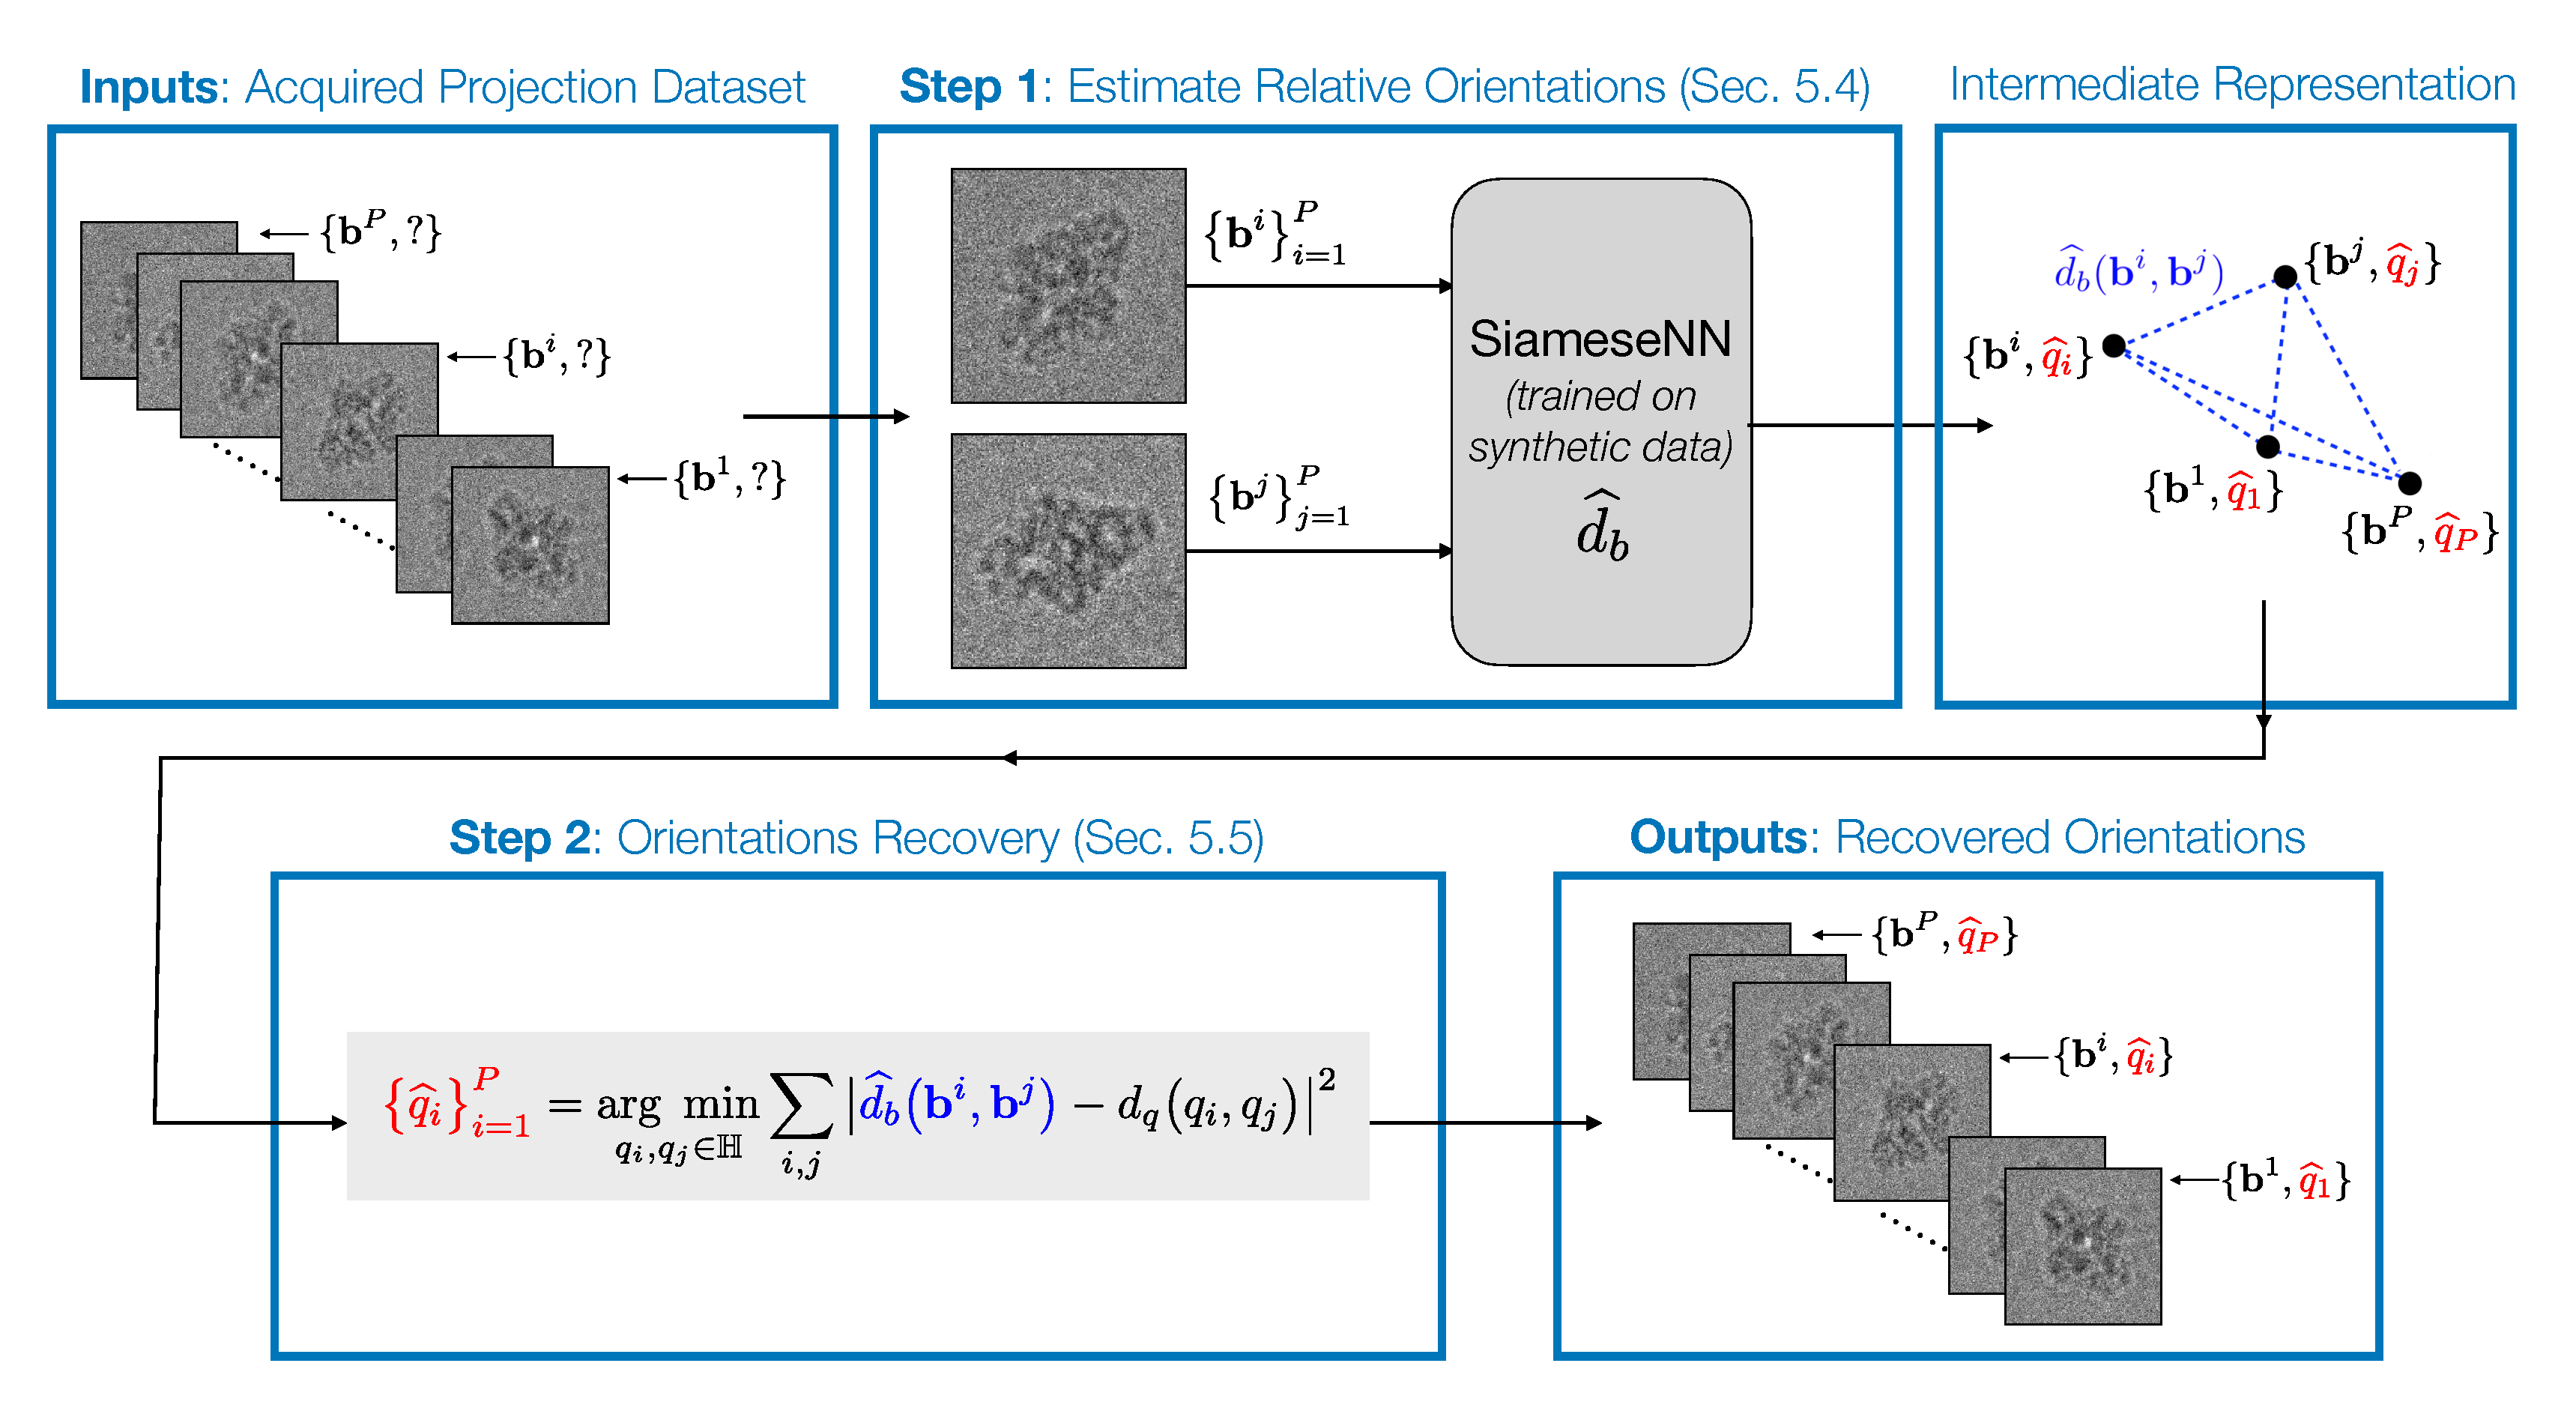
\includegraphics[width=\textwidth]{schematic_overview}
    \caption{
        \textbf{Overview of the proposed method.}
        We denote the $i$th projection by $\mathbf{p}_i$ and its orientation by $q_i$. The distance between two orientations is denoted by $d_q$, and the estimated distance between two projections by $\widehat{d}_p$; the latter is implemented as a SiameseNN.
        Our method consists of two steps: (i) estimate distances between pairs of projections, and (ii) recover orientations from the estimated distances.
        % Our method effectively (i) estimates a metric space, then (ii) embed it in the space of 3D orientations, $\SO(3)$.
        \todo{Update sections in figure.}
        \todo{Update titles: Step 1: estimate distances. Step 2: recover orientations.}
        \mdeff{It would be amazing to have a visual of the embedding made in step 2: finding points in SO(3) such that the geodesic distances between them are the estimated distances. As we can't see SO(3) / $S^3$, we could try with $S^2$, which is a subset/projection.} \lau{I'll change the notations in the figure once we have settle on the final ones.}
    }
    \label{fig:schematic:overview}
\end{figure}

We present a method that learns to estimate the unknown orientation associated to each projection in a single-particle cryo-EM dataset without relying on any intermediate reconstruction procedure. Our approach relies on the well-know observation that the greater the similarity between two 2D projections, the more likely they originated from two 3D particles that adopted close orientations in the ice layer prior to imaging\footnote{Up to protein symmetries, which we discuss later.}; this principle guides a number of applications in the field~\cite{frank2006three}.

Taking this line of thought further, we propose to train a function---parametrized as a neural network---to predict the relative orientation between two projections based on their similarity. This trained network then allows us to estimate, for any new projection dataset, the relative orientations between pairs of its projections. From these estimated distances, we then retrieve the orientation for each projection through an appropriate minimization scheme. Our two-steps method is illustrated in \figref{schematic:overview}. 

%to embed it on the space of 3D orientations, $\SO(3)$.
% In practice, our method consists of: (i) estimate the distance between pairs of projections, and (ii) recover
% \mdeff{maybe too repetitive with figure caption}


\paragraph{Distance Learning}
The resort to a neural network to estimate the relative distances is driven by several reasons. First, and most obviously, this information is not directly accessible from the dataset itself. To circumvent this, we rely on the postulate that the similarity between two projections is a good proxy for their relative orientation, for some appropriate meaning of similarity. The ``handcrafting'' of a metric that would robustly predict these distances is an intricate---if not impossible---task, partly because the invariants are difficult to specify. Hence, we rather opt to \textit{learning} this distance function by parametrizing it as a neural network. For its training, we capitalize on i) the public availability of numerous 3D atomic models\footnote{\texttt{https://www.ebi.ac.uk/pdbe/emdb}} and ii) our ability to model the cryo-EM imaging procedure in order to generate realistic cryo-EM projection datasets. 

%If the distances are exact geodesic distances between orientations, then orientation recovery will find a perfect realization of the metric space, with zero error.
%In practice, distances estimated from projections will only be a proxy of true distances.
%Experiment \secref{results:orientation-recovery:sensitivity} shows that a lower distance estimation error translates to a lower orientation recovery error.

\paragraph{Orientation Recovery}
The task of recovering points based on their relative distances has been extensively studied in the literature, primarily within the frameworks of dimensionality reduction and data visualization~\cite{belkin2003laplacian,kruskal1978multidimensional, maaten2008visualizing, mcinnes2018umap,dokmanic2015euclidean}. 
These methods aim at mapping high-dimensional data onto a lower-dimensional space in such a way that the structure of the metric space is preserved. 
Formally, the recovery is achieved by minimizing an appropriate loss function; well-known examples include Laplacian eigenmaps, multi-dimensional scaling (MDS), Isomap, LLE, t-SNE, and UMAP. 
In the Euclidean setting, the embedding of distance matrices (given by their eigenvectors) is especially well-described.
In particular, the framework of the Euclidean distance matrices (EDMs)~\cite{dokmanic2015euclidean} provides theoretical guarantees on the retrieval of points from collected distances.

In our case, as we shall shortly explain, we aim to perform the embedding on $\SO(3)$, the non-Euclidean space of 3D rotations. Hence, the loss function to minimize (\secref{method:orientation-recovery}) is non-convex. Furthermore, we are not aware of any theoretical characterization of its behaviour when input distances are lacking or corrupted by perturbations. That being said, the locally-Euclidean behavior of the $\SO(3)$ space offers some hope on the feasibility of this minimization. 
Indeed, despite the lack of theoretical guarantees, we are able to appropriately minimize our loss function using a gradient-based algorithm, as we experimentally demonstrate in \secref{results:orientation-recovery:exact}.

%%%%%%%%%%%%%%%%%%%%%%%%%%%%%%%%%%%%%%%%%%%

%\subsection{Unit Quaternions and the Geodesic Distance}
%\subsection{Representation of orientations}
\subsection{Representation of orientations}\label{sec:method:orientation-representation}

Inside the electron microscope, each 3D particle is positioned at a given orientation with respect to the detector plane $\bsy=(y_1,y_2)\in \mathbb{R}^2$, as illustrated in Figure~\ref{fig:imaging-geometry} (left). Hence, for each particle, the geometry of the imaging procedure is described by the geometrical transformation that maps its object coordinate system $(x_1,x_2,x_3)$ to the measurement coordinate system $(y_1,y_2)$. This mapping corresponds to a rotation in $\SO(3)$, the group of all 3D rotations about the origin of $\mathbb{R}^3$; in that space, every rotation can be described by a $3\times3$ orthogonal matrix with determinant~$1$. 

The standard approach in single-particle cryo-EM is to use Euler angles to parametrize the rotation matrix that relates the two coordinate systems~\cite{sorzano2014interchanging}. The Euler angles, denoted as $\bth=(\theta_1,\theta_2,\theta_3)\in [0;2\pi)\times [0;\pi] \times [0;2\pi)$, are a set of three angles that describes a sequence of three rotations about three fixed axes (Figure~\ref{fig:imaging-geometry} (right)). 
Unfortunately, the geodesic distance between two rotations $\mathbf{R}(\bth_1)$, $\mathbf{R}(\bth_2)\in \SO(3)$ parametrized by Euler angles cannot be directly computed from $\bth_1$, $\bth_2$.
It requires the computation of the rotation matrices, which is computationally inefficient\footnote{Another technical challenge with Euler angles is that they suffer from the so-called gimbal lock problem, which arises when $\theta_2=0$ and restricts the number of rotational degrees of freedom to one even though $\theta_1$ and $\theta_3$ have not yet been fixed~\cite{koks2006explorations}.}.

As our method requires the repeated computation of the geodesic distance, we resort to a more convenient representation of 3D rotations that relies on unit quaternions $q\in\mathbb{U}$, with  $\mathbb{U}=\big\{q\in\mathbb{H} \; \, | \; \,\lvert q \rvert =1\big\}$, which identify the $\mathbb{S}^3$ hypersphere in  $\mathbb{R}^4$, and concisely represent the elements of the $\SO(3)$ group. The geodesic distance $d_q:\mathbb{U}\times\mathbb{U}\rightarrow [0,\pi]$ between two unit quaternions $q_i, q_j\in\mathbb{H}$ is then defined as
\begin{equation}
    d_q(q_i, q_j) = 2 \arccos \big(| \langle q_i, q_j \rangle| \big),
    \label{eqn:distance:orientations}
\end{equation}
with $\langle q_i, q_j \rangle$ the inner product between two quaternions.
The distance~\eqnref{distance:orientations} is the shortest distance between $q_i$ and $q_j$ on the surface of $\mathbb{S}^3$.

As $\mathbb{S}^3$ is isomorphic to the universal cover of $\SO(3)$, the geodesic distance corresponds to the magnitude of the relative orientation $\mathbf{R}_*$ between $\mathbf{R}(q_i)$ and $\mathbf{R}(q_j)$ in $\SO(3)$~\cite{huynh2009metrics}.
In other words, the relative distance between two rotations encoded by unit quaternions can be efficiently computed from the unit quaternions themselves through~\eqnref{distance:orientations}, which is of key practical importance for this work.

%For the sake of conciseness, we shall use the term ``with orientation~$q$'' to refer to 2D/3D objects considered in an imaging geometry parametrized by $q$.

%%%%%%%%%%%%%%%%%%%%%%%%%%%%%%%%%%%%%%%%%%%

\subsection{Distance learning}%\label{sec:method:distance-learning}
%\subsection{Metric learning}%\label{sec:method:distance-learning}
%\subsection{Estimating Relative Orientations from Projections}
%\subsection{Relative orientation estimation}
%\subsection{Relative orientation estimation from projections}

%We capitalize on the powerful function approximation capabilities of neural networks and on our ability to faithfully model the cryo-EM imaging process for the generation of training data.

%To make such training possible, we capitalize on our ability to model the cryo-EM imaging procedure to generate a large, representative synthetic dataset using publicly available 3D atomic models.
%Once the distance learned, it can be used in the aforementioned two-steps method (see \figref{schematic:overview}) for any projection dataset.

The goal is to train a function---parametrized as a neural network---to predict the relative orientation between two projections based on their similarity. \figref{schematic:distance-learning} illustrates the proposed learning paradigm.

\begin{figure}
    \centering
    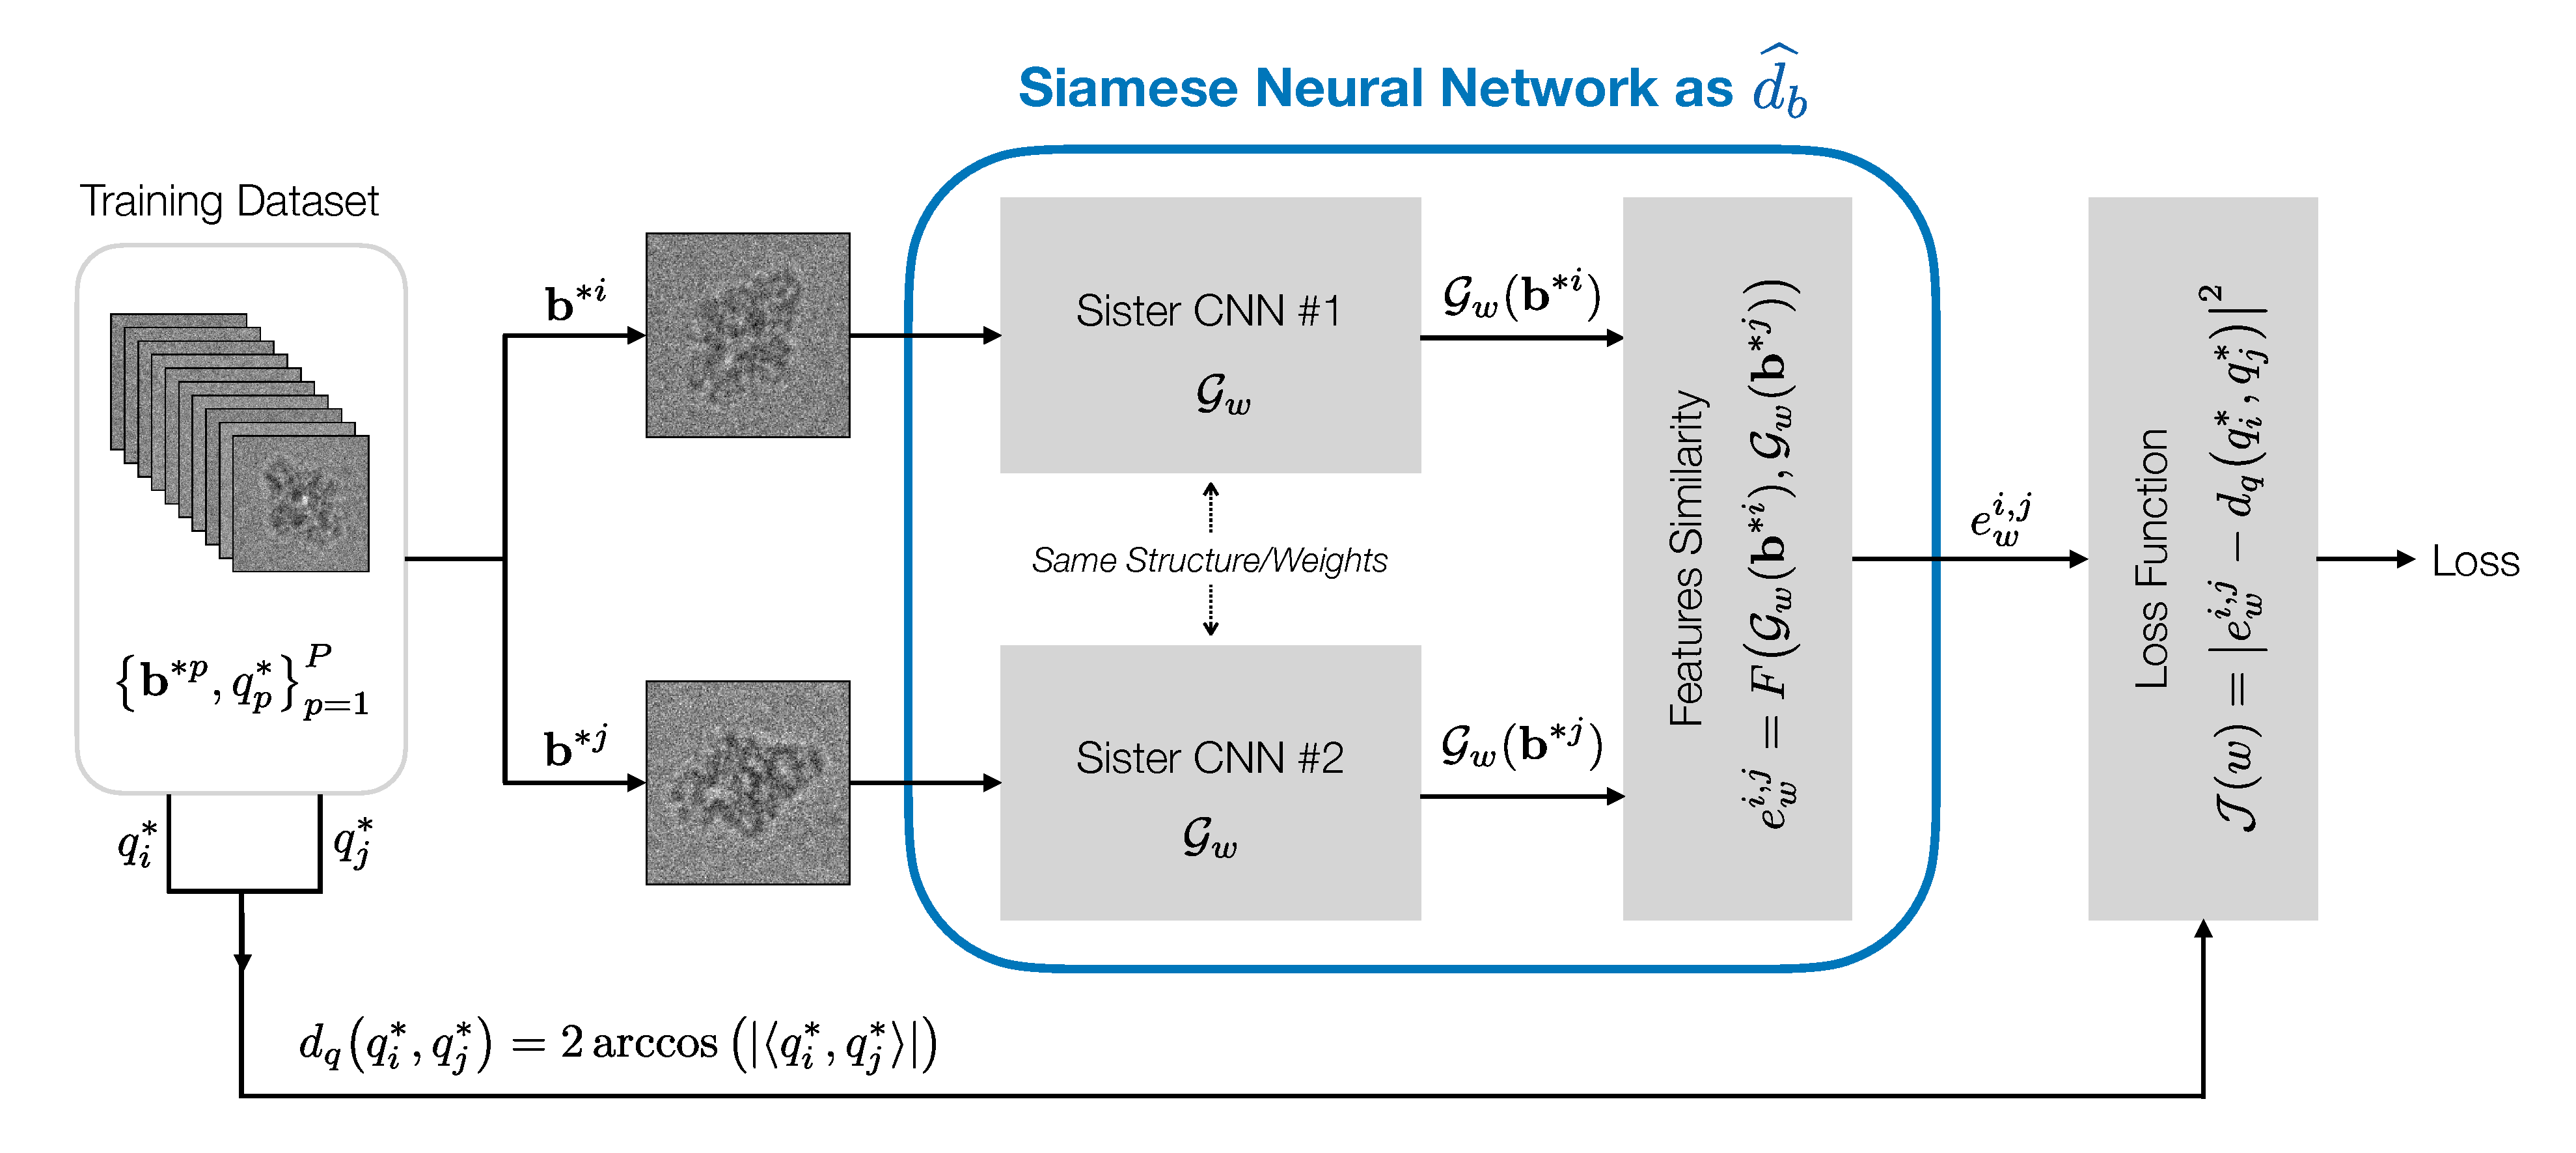
\includegraphics[width=\textwidth]{schematic_siamese}
    \caption{
        We are looking for a distance $d_p$ between projections that is an accurate estimator of the distance $d_q$ between their orientations.
        We propose to parameterize $d_p$ as a Siamese neural network (SiameseNN), trained on a synthetic dataset of $P \approx 10^3$ projections with associated orientation.
        \todo{Figure: feature distance (not similarity) $d_f$ is \eqnref{distance:projections}. Loss function is \eqnref{distance-learning}. "Same Structure/Weights" $\rightarrow$ "Same NN $\G$ and shared weights $w$".}
}
    \label{fig:schematic:distance-learning}
\end{figure}

From a training dataset $\{ \mathbf{p}_{i}, q_i\}_{i=1}^{P}$ made of $P$ projections $\p_i \in \R^{n_p}$ with associated orientation $q_i \in \U$, we learn the \textit{projection distance}
\begin{equation}
    \widehat{d}_p = \argmin_{d_p} \sum_{i,j} \left| d_p\big(\mathbf{p}_{i},\mathbf{p}_{j}\big) - d_q\big(q_i,q_j\big) \right|^2,
    \label{eqn:distance-learning}
\end{equation}
with $d_q$ defined in~\eqnref{distance:orientations}.
The distance $d_p$ is parameterized as the Siamese neural network (SiameseNN)~\cite{chopra2005learning}
\begin{equation}
    d_p(\p_i, \p_j) = d_f(\G_w(\p_i), \G_w(\p_j)),
    \label{eqn:distance:projections}
\end{equation}
where $\G_w$ is a convolutional neural network with weights $w$ that is trained to extract the most relevant features $\f_i \in \R^{n_f}$ from a projection $\p_i$. SiameseNNs, also termed ``twin networks'', are commonly used in the field of deep metric learning to learn similarity functions~\cite{yi2014deep}. 
The distance in the feature space $d_f$ is often taken to be the Euclidean distance $d_f(\f_i, \f_j) = \Vert \f_i - \f_j \Vert_2$.
To facilitate the learning of a distance that respects the elliptic geometry of $\U$, we set $d_f = d_q$.


Evaluating the sum in \eqnref{distance-learning} requires $P^2$ distance evaluations.
As this is computationally intractable for cryo-EM datasets with typically $P \approx 10^5$ projections, we sample only a subset of pairs.
In practice, \eqnref{distance-learning} is minimized by stochastic gradient descent (SGD) over small batches of pairs, with weight updates computed by back-propagation of the error.
% error / objective value

%%%%%%%%%%%%%%%%%%%%%%%%%%%%%%%%%%%%%%%%%%%

\subsection{Orientation recovery}\label{sec:method:orientation-recovery}
%\subsection{Orientation recovery from relative orientations}

Equipped with a trained estimator $\widehat{d}_p$, we then recover the orientations from a set of projections $\big\{ \mathbf{p}_k \big\}_{k=1}^P$ through 
\begin{equation}
    \big\{ \widehat{q}_k \big\}_{k=1}^P = \argmin_{q_i, q_j \in \U} \sum_{i,j} \left| \widehat{d}_p \left( \p_i, \p_j \right) - d_q\left(q_i,q_j\right) \right|^2.
    \label{eqn:orientation-recovery}
\end{equation}
Note that the sole difference with~\eqnref{distance-learning} is that the minimization is performed over the projections $q_i$ rather than the distance $d_p$. Here again, the sum in \eqnref{orientation-recovery} is sampled for computational reasons.
A strategy, commonly employed by \todo{those classic algos}, that amounts to build and embed a sparse distance graph. \lau{@Mdeff: Can you please fill here? Thanks.}
In practice, \eqnref{orientation-recovery} is also minimized by mini-batch SGD.
%We experimentally demonstrate in \secref{results:orientation-recovery:exact} that both approximations don't affect recovery performance.
